% Source problem: 2012ap_exam.pdf, PDF pp. 2--3.
\documentclass[11pt,a4paper]{article}
\usepackage[margin=24mm]{geometry}
\usepackage{fontspec}
\usepackage{xeCJK}
\setCJKmainfont{HaranoAjiMincho-Regular.otf}
\setCJKsansfont{HaranoAjiGothic-Medium.otf}
\usepackage{amsmath,amssymb}
\usepackage{tikz}
\usetikzlibrary{arrows.meta}
\setlength{\parindent}{1em}
\setlength{\parskip}{0.35em}
\renewcommand{\figurename}{図}
\title{物理工学専攻 院試解答集\\2012年 物理学I 第1問}
\author{政岡凜太郎}
\date{}
\begin{document}
\maketitle

\section*{[1] 円柱Bにはたらく摩擦}
円柱Bの中心を原点に取り、右向きを $x$ 軸正方向とする。円柱CからBが受ける接線摩擦力 $F$ は接触点で左下向き、床からの摩擦力 $F'$ は床面に沿って左向きである。CからBへの法線力を $T$、床からBへの法線力を $N$ とすると、Bに作用する力は次のようになる。
\begin{figure}[htbp]
\centering
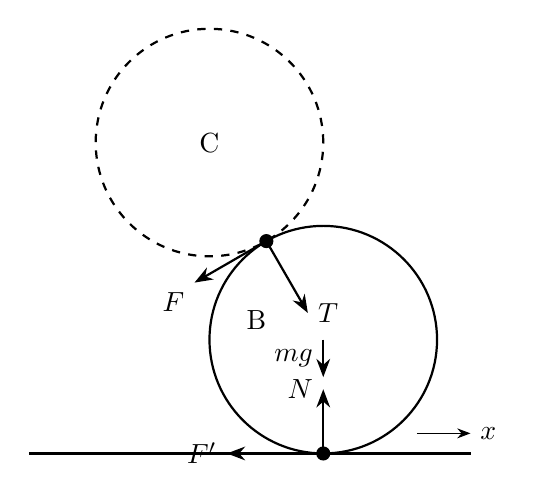
\begin{tikzpicture}[>=Stealth,scale=1.7]
  % Illustration units: a=0.85.  The upper centre follows |BC|=2a.
  \def\a{0.85}
  \pgfmathsetmacro{\rtthree}{sqrt(3)}
  \coordinate (B) at (0,0);
  \coordinate (C) at (-\a,{\rtthree*\a});
  \coordinate (P) at ({-\a/2},{\rtthree*\a/2});
  \coordinate (Q) at (0,-\a);
  \draw[thick] (B) circle (\a);
  \draw[thick,dashed] (C) circle (\a);
  \node at (-0.5,0.15) {B};
  \node at (-\a,{\rtthree*\a}) {C};
  \draw[thick] (-2.2,-\a)--(1.1,-\a);
  \fill (P) circle (1.5pt);
  % Exact unit directions from the centre-line normal and tangent.
  \draw[->,thick] (P)--++({-0.62*\rtthree/2},{-0.62/2}) node[below left] {$F$};
  \draw[->,thick] (P)--++({0.62/2},{-0.62*\rtthree/2}) node[right] {$T$};
  \fill (Q) circle (1.5pt);
  \draw[->,thick] (Q)--++(-0.72,0) node[left] {$F'$};
  \draw[->,thick] (Q)--++(0,0.48) node[left] {$N$};
  \draw[->,thick] (B)--++(0,-0.28) node[midway,left] {$mg$};
  \draw[->] (0.7,-0.7)--(1.1,-0.7) node[right] {$x$};
\end{tikzpicture}
\caption{円柱Bの自由物体図。摩擦力は各接触面の接線方向。}
\end{figure}

Bの中心軸まわりでは、Cとの接触摩擦と床摩擦が腕の長さ $a$ で逆向きのトルクを作る。静止しているので
\begin{equation}
  \boxed{F=F'.}
\end{equation}

\section*{[2] 静止に必要な摩擦係数}
左右対称なので、CがA、Bから受ける接触力の鉛直成分を合計すると
\begin{equation}
  2\left(\frac{F}{2}+\frac{\sqrt3}{2}T\right)=mg,
  \qquad F+\sqrt3T=mg.
\end{equation}
Bの水平方向の釣合いは
\begin{equation}
  -F'-\frac{\sqrt3}{2}F+\frac12T=0.
\end{equation}
$F'=F$ と連立して
\begin{equation}
  F=F'=\frac{2-\sqrt3}{2}mg,\qquad T=\frac12mg.
\end{equation}
Bの鉛直釣合いから床の法線力は
\begin{equation}
  N=mg+\frac12F+\frac{\sqrt3}{2}T=\frac32mg.
\end{equation}
よって、円柱間と床面でそれぞれ静止摩擦力が最大静止摩擦力を越えないための条件は
\begin{equation}
  \boxed{\mu\geq\frac FT=2-\sqrt3,\qquad
         \mu'\geq\frac{F'}{N}=\frac{2-\sqrt3}{3}.}
\end{equation}
等号は最大静止摩擦力が働く限界の状態を表し、この場合も静止の条件に含まれる。

\section*{[3] 円柱の慣性モーメント}
円柱の体積密度は $m/(\pi a^2l)$。中心軸から距離 $r$ の薄い円筒殻の質量は $2\pi rl\,dr$ に密度を掛けたものだから
\begin{align}
  I&=\int_0^a r^2\frac{m}{\pi a^2l}(2\pi rl)\,dr
   =\frac{2m}{a^2}\int_0^a r^3\,dr\\
   &=\boxed{\frac12ma^2}.
\end{align}

\section*{[4] 位置Tまでの運動}
右向きを正、反時計回りを正とする。床接点の床に対する速度は $v+a\omega$ で、初期値は $v_0+a\omega_0>0$ である。
この速度が初めて0になるまでは接点が右へ滑るので、動摩擦力は左向きで大きさ $\mu''mg$ となる。
以下の滑走中の式はこの区間に適用する。摩擦は並進速度を減らし、反時計回りの角速度も減らす。
\begin{equation}
  m\dot v=-\mu''mg,\qquad I\dot\omega=-a\mu''mg.
\end{equation}
$I=ma^2/2$ を使い初期条件を入れると
\begin{equation}
  v(t)=v_0-\mu''gt,\qquad
  \omega(t)=\omega_0-\frac{2\mu''g}{a}t.
\end{equation}
重心が一時停止する位置Tでは $t_T=v_0/(\mu''g)$ なので
\begin{equation}
  \boxed{ST=v_0t_T-\frac12\mu''gt_T^2=\frac{v_0^2}{2\mu''g}},
  \qquad
  \boxed{\omega(T)=\omega_0-\frac{2v_0}{a}}.
\end{equation}

\section*{[5] 滑らずに転がり始める速さ}
床との相対速度がゼロになる条件は、床接点の速度 $v+a\omega=0$。滑走中
\begin{equation}
  v(t)+a\omega(t)=v_0+a\omega_0-3\mu''gt
\end{equation}
だから、転がり開始時刻は
\begin{equation}
  t_R=\frac{v_0+a\omega_0}{3\mu''g}.
\end{equation}
そのときの符号付き重心速度は
\begin{equation}
  v_R=v_0-\mu''gt_R=\frac{2v_0-a\omega_0}{3}.
\end{equation}
問題の[6]の状況では $t_R>t_T$ であり、$v_R<0$。従って速さは
\begin{equation}
  \boxed{|v_R|=\frac{a\omega_0-2v_0}{3}}.
\end{equation}

\section*{[6] 位置Sへ戻る条件}
転がり始めるのがT通過より後であるには $t_R>t_T$。滑走だけを続けた場合にSへ戻る時刻は $t_S=2v_0/(\mu''g)$ であり、Sに達する前に滑りが止まるには $t_R<t_S$。したがって
\begin{equation}
  \frac{v_0}{\mu''g}<\frac{v_0+a\omega_0}{3\mu''g}
   <\frac{2v_0}{\mu''g}.
\end{equation}
$v_0,\mu'',g,a>0$ を用いて整理すると
\begin{equation}
  \boxed{\frac{2v_0}{a}<\omega_0<\frac{5v_0}{a}}.
\end{equation}
この範囲ではTの後に左向きの無滑り運動へ移り、Sまでの距離を等速で戻る。

\end{document}
